%
%  $Description: Author guidelines and sample document in LaTeX 2.09$ 
%
%  $Author: ienne $
%  $Date: 1995/09/15 15:20:59 $
%  $Revision: 1.4 $
%

\documentclass[10pt,twocolumn]{article} 
\usepackage{latex8}
\usepackage{times}
\usepackage{graphicx}
\usepackage{subcaption}
\usepackage{algorithm}
\usepackage{algorithmic}
\usepackage{adjustbox}
\usepackage{enumitem}
\usepackage{hyperref}
\usepackage{cite}

\title{Differential Analysis of LLMs in Text2SQL Generation}

\author{Jaykumar Patel\\
patel.jay4802@utexas.edu\\
% For a paper whose authors are all at the same institution, 
% omit the following lines up until the closing ``}''.
% Additional authors and addresses can be added with ``\and'', 
% just like the second author.
\and
An-Jung Huang\\
ajhuang@utexas.edu\\
\and
Ryan Kolm\\
ryankolm@utexas.edu\\
}

\begin{document}

\maketitle

\begin{abstract}

Large Language Models (LLMs) have shown remarkable capabilities in translating natural language questions into executable SQL queries, a task known as Text2SQL. In this work, we conduct a systematic evaluation of several state-of-the-art LLMs and two distinct Text2SQL frameworks: agentless and agent-based pipelines. Our experiments assess accuracy, consistency, and execution robustness on the BIRD-SQL Dev Set. By enabling users to query structured databases through natural language, effective Text2SQL systems have the potential to democratize data access, allowing non-developers to retrieve complex information from structured databases without needing specialized technical skills. Our study aims to inform future design choices for building more reliable and accessible natural language interfaces to databases.
        
% We find that model choice and framework design substantially influence both the correctness and reliability of generated SQL, with trade-offs between simplicity, performance, and interpretability. Our results provide actionable insights for practitioners building natural language interfaces to databases, and highlight open challenges in making Text2SQL systems more dependable in real-world applications.

\end{abstract}

\section{Introduction}

As large language models (LLMs) continue to envolve and improve, an interesting application of LLMs is in the generation of SQL queries from natural language. This is known as Text2SQL. Text2SQL can enable non-experts to extract valuable information from a database without having to learn complex query languages like SQL. By simply describing the data they want in plain English, users can leverage LLMs to translate their requests into structured queries that interact directly with a database. This has the potential to democratize data access across organizations, reduce reliance on technical teams for routine data retrieval tasks, and improve overall efficiency in data-driven decision-making.

In this project, we compare the performance of different LLMs in generating SQL queries from natural language. We explore 2 different frameworks, agentless and agent-based, and 3 different LLMs, Claude 3.5 Sonnet, GPT-4o mini, and Llama3.1 8B. In the agentless framework, the descriptions of all tables in the database (relevant and irrelevant) are passed as context to the LLM when generting the SQL query given the natural language query. In the agent-based framework, there are 3 agents that handle specific tasks such as determining the number of relevant tables, retrieving the descriptions of the relevant tables, and generating a SQL query given a natural language query. We run our agentless and agent-based frameworks with the 3 different LLMs on the BIRD-SQL Dev Set benchmark. 

By systematically analyzing various LLMs and frameworks, we aim to understand how model choice and pipeline design impact the accuracy, consistency, and execution success of generated SQL queries. Our findings can help guide the development of more reliable and accessible Text2SQL systems, ultimately making database interaction easier and more intuitive for a broader range of users.

\section{Previous Work}

Text2SQL has been an active area of research, with approaches evolving alongside advances in natural language processing. Early methods primarily relied on rule-based systems \cite{rule-based} and semantic parsing \cite{semantic-parsing}, which required significant domain-specific engineering and struggled to generalize across different database schemas. With the rise of deep learning, encoder-decoder architectures and pre-trained language models began to dominate, enabling more flexible mappings from natural language to SQL queries.

Recent work has explored building Text2SQL pipelines that leverage LLMs to generate SQL queries through structured multi-step processes. CHASE-SQL \cite{chase-sql} and XiYan-SQL \cite{xiyan-sql} both implement multi-agent frameworks in which one agent retrieves relevant schema information, another generates candidate queries, and a final agent selects the most appropriate SQL statement. CHASE-SQL employs methods such as divide-and-conquer chain-of-thought (CoT) reasoning, query-plan-based CoT reasoning, and online synthetic example generation to enhance candidate generation. In contrast, XiYan-SQL integrates supervised fine-tuning of multiple specialized generators alongside in-context learning (ICL) with skeleton-based example selection to produce high-quality and diverse SQL candidates. CHASE-SQL and XiYan-SQL rank 2nd and 4th respectively for the BIRD benchmark.

While these recent frameworks demonstrate the effectiveness of multi-agent pipelines for improving Text2SQL performance, there remains value in systematically comparing different LLMs and framework designs under a common experimental setting. In this work, we conduct an empirical evaluation of both agentless and agent-based pipelines across multiple LLMs, aiming to better understand how model choice and pipeline structure influence SQL generation quality on the BIRD-SQL Dev Set. Specifically, we evaluate not only a larger model such as Claude 3.5 Sonnet, but also smaller, potentially more economical models like GPT-4o Mini and Llama 3.1 8B. To keep the evaluation feasible, we employ a simplified version of the agent-based framework, utilizing a single generator rather than multiple specialized generators. Additionally, to assess the consistency of each model and framework combination, we run each configuration three times.


\section{Methodology}

In this section, we outline the methodology used for our differential analysis of LLMs in Text2SQL generation.

\subsection{Model Selection}

For this study, we selected the three Large Language Models (LLMs) Claude 3.5 Sonnet, GPT-4o mini, and Llama3.1 8B. These models for their widespread adoption and diversity in model size. Particularily, Claude 3.5 Sonnet has ~175 billion parameters; whereas, GPT-4o mini and Llama3.1 8B have ~8 billion parameters \cite{model-size}. Notably, Llama3.1 8B is open-source, while GPT-4o Mini and Claude 3.5 Sonnet are closed-source. By comparing these models, we aim to evaluate how performance varies not only with model size but also between open-source and closed-source LLMs.

Temperature controls the degree of randomness in the text generated by large language models during inference (https://www.ibm.com/think/topics/llm-temperature). The default temperature for Claude 3.5 Sonnet is 1.0, which represents the maximum level of randomness. For GPT-4o mini, the default temperature is 0.7; however, in this study, we increase it to 1.0 to encourage greater diversity in the SQL queries generated across three runs, thereby improving the chances of obtaining a correct result. For Llama 3.1 8B, we retain the default lower temperature, as smaller models are generally more prone to hallucinations when exposed to higher levels of randomness.

\subsection{Framework Selection}

There are many ways that Text2SQL can be implemented. In this study, we compare the performance difference between 2 frameworks, one that performs without AI agents (agentless) and one that utilizes a series of AI agents (agent-based).
\begin{enumerate}
    \item \textbf{Agentless}: In this framework, an LLM is used to generate the response directly. The NLQ and all table descriptions are provided to the \textbf{LLM}. The LLM then generates a SQL query. The agentless pipeline can be seen in Figure \ref{fig:agentless-pipeline}.
    
    \item \textbf{Agent-based}: In this framework, there are distinct agents that each play a different role in the generation of the response. Before this pipeline can be used, all table descriptions must be vectorized and stored in \textbf{ChromaDB}. There are three agents: the \textbf{Relevance Agent}, \textbf{Retrieval Agent}, and \textbf{Query Agent}. The NLQ and all table descriptions are provided to the \textbf{Relevance Agent}, which determines the number of tables that are relevant, denoted as $K$. Then, the \textbf{Retrieval Agent} retrieves the $K$ table descriptions from ChromaDB that are most similar to the NLQ. This process is similar to the retrieval step in a RAG system and allows us to obtain the relevant table descriptions. Finally, the NLQ and the retrieved table descriptions are provided to the \textbf{Query Agent}, which is responsible for generating the SQL query. The agent-based pipeline can be seen in Figure \ref{fig:agent-based-pipeline}.
\end{enumerate}


\begin{figure}[h]
    \centering
    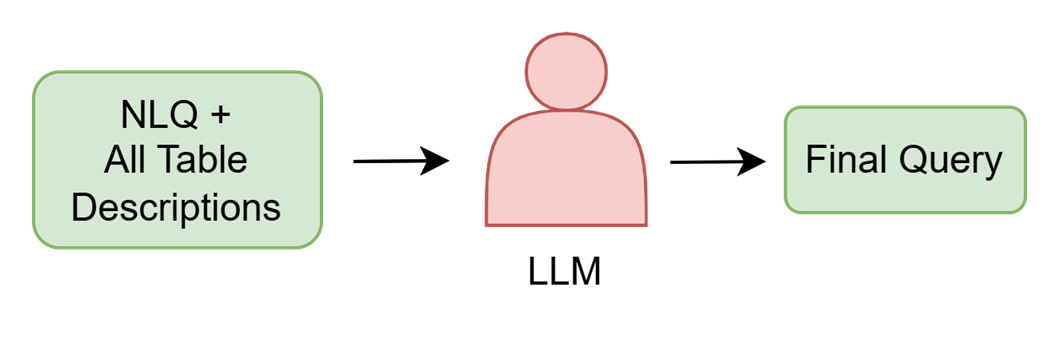
\includegraphics[width=0.45\textwidth]{imgs/Agentless Pipeline.png}
    \caption{Agentless Text2SQL Pipeline}
    \label{fig:agentless-pipeline}
\end{figure}

\begin{figure}[h]
    \centering
    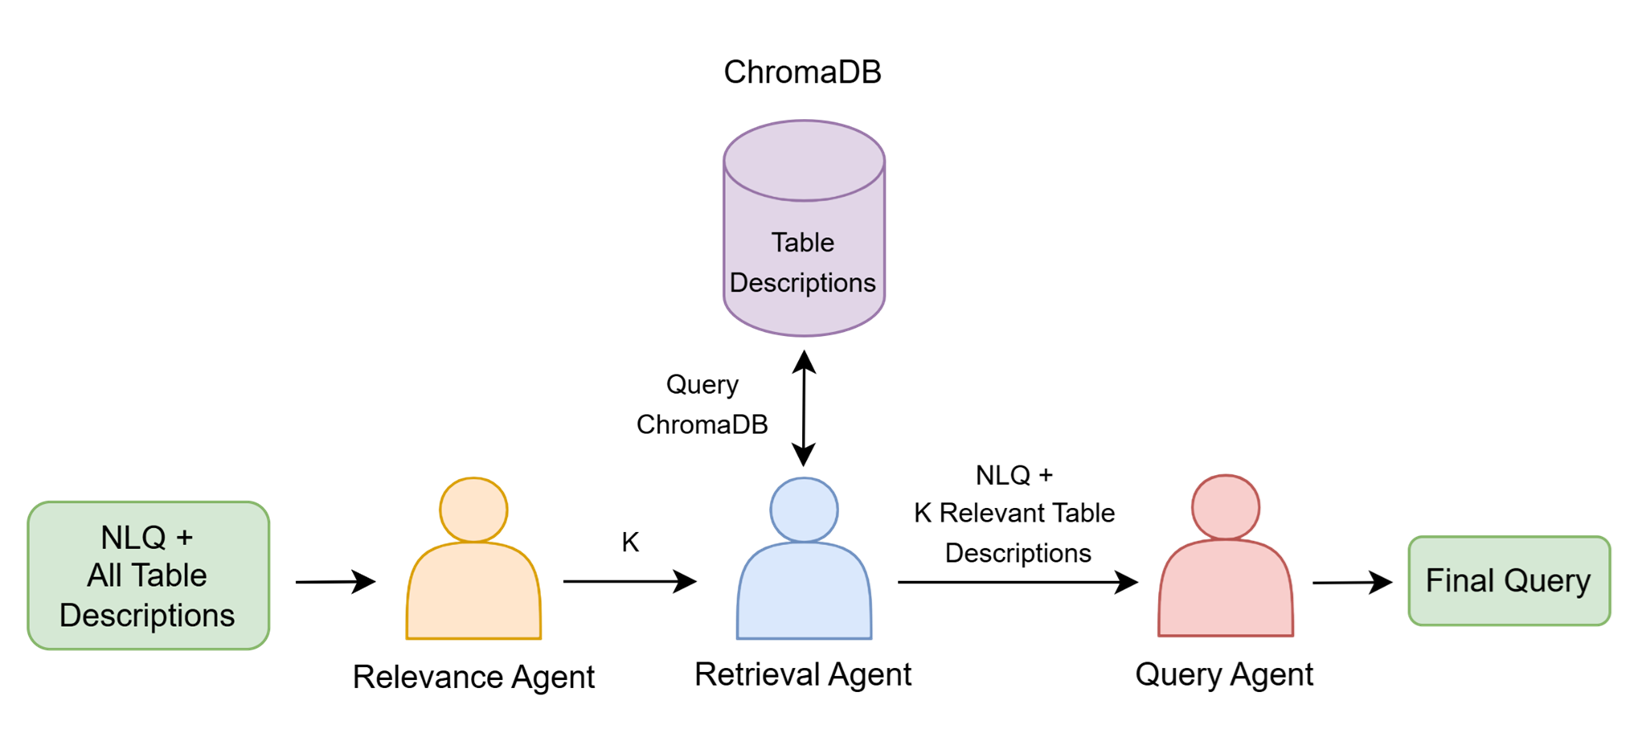
\includegraphics[width=0.45\textwidth]{imgs/Agent-based Pipeline.png}
    \caption{Agent-based Text2SQL Pipeline}
    \label{fig:agent-based-pipeline}
\end{figure}

The main difference between the agentless and agent-based frameworks lies in the Text2SQL generation phase of the pipeline: agentless uses the descriptions of all tables, whereas agent-based selectively uses only the descriptions of relevant tables. Comparing these two frameworks provides insight into the trade-offs between simplicity and modularity, particularly in terms of scalability and accuracy---considering that agentless requires fewer LLM calls than agent-based. Specifically, we aim to explore whether introducing specialized agents leads to more accurate query generation, or if the added complexity results in diminishing returns compared to a simpler, monolithic approach. This evaluation can help guide the future development of LLM-powered database interfaces.

Our agent-based pipeline design is also inspired by patterns observed in leading multi-agent Text2SQL frameworks, such as CHASE-SQL and XiYan-SQL. These approaches typically organize the generation process into three main phases: (1) a schema or value retrieval phase to provide database context, (2) a candidate generation phase to produce potential SQL queries, and (3) a candidate selection phase to choose the best query among multiple options. Our pipeline similarly incorporates the first two phases: we employ a Relevance Agent and a Retrieval Agent to retrieve and focus the relevant table descriptions, followed by a Query Agent to generate the final SQL query. However, because we generate only a single candidate query per NLQ, a selection phase is not necessary, as there are no multiple candidates to choose from. This streamlines the pipeline and keeps the experimental setup simple.

An important motivation for exploring agentless and agent-based frameworks is the ``lost in the Middle" effect \cite{lostinmiddle}, where LLMs struggle to effectively utilize relevant information when it is in the middle of large contexts. As the context grows---particularly with many irrelevant table descriptions---LLMs can become less precise in their reasoning if the relevant information gets ``lost" in the context. The agent-based framework addresses this by employing dedicated agents to retrieve and focus only on the most relevant table descriptions, thereby reducing context size, mitigating the ``Lost in the Middle" effect, and potentially improving the model's ability to generate accurate SQL queries.


\subsection{Benchmark Dataset Selection}

For this study, we use the \href{https://bird-bench.github.io/}{BIRD-SQL Dev Set} as the benchmark for evaluation. BIRD-SQL is a widely adopted benchmark in the Text2SQL community, known for its diverse database schemas, realistic query complexity, and standardized difficulty categorizations (simple, moderate, and challenging). Its acceptance as a standard benchmark enables fair comparisons across different methods and models. 

The BIRD-SQL Dev Set includes table descriptions for every database, a collection of natural language questions (NLQs), their corresponding ground-truth SQL queries, and assigned difficulty levels. For our experiments, we focus on the ``student-club" database and sample 30 questions, comprising 18 simple, 9 moderate, and 3 challenging examples. This curated subset serves as the ground truth against which we evaluate the performance of the selected LLMs and frameworks.

\subsection{Evaluation Metrics}

We evaluate the performance of each Model+Framework combination across three main metrics: \textbf{correctness}, \textbf{consistency}, and \textbf{execution error rate}.

\begin{itemize}
    \item \textbf{Correctness} measures how often the generated SQL query produces the correct result for a given natural language question (NLQ). To assess accuracy, we execute the generated SQL query and the corresponding ground-truth SQL query from BIRD-SQL on the database, and determine correctness by comparing their execution results. A generated query is considered correct if its execution result exactly matches the execution result of the ground-truth query. We categorize accuracy based on the number of successful generations out of three attempts for each query: 0/3, 1/3, 2/3, or 3/3 correct generations.
    \item \textbf{Consistency} captures the stability of a model's outputs across multiple runs. A Model+Framework combination that achieves 3/3 correct generations for a query is considered highly consistent, while fluctuating results (e.g., 1/3 or 2/3 correct) indicate lower consistency.
    \item \textbf{Execution Error Rate} is the percentage of generated SQL queries that fail to execute, typically due to syntax errors, invalid table references, or improper SQL structure. A lower execution error rate reflects greater robustness and syntactic reliability. A higher execution error rate may indicate hallucinations, misunderstandings of the database schema, or general instability in query generation.
\end{itemize}

Additionally, we compare the overall performance between the agentless and agent-based frameworks to explore the trade-offs between simplicity (agentless) and modular specialization (agent-based). Each Model+Framework combination is tested on the 30 sampled queries, with three independent runs per query to capture variability.

\section{Results}

\subsection{Accuracy and Consistency}
 
\begin{figure}[h]
    \centering
    % First subfigure
    \begin{subfigure}[b]{0.45\textwidth}
        \centering
        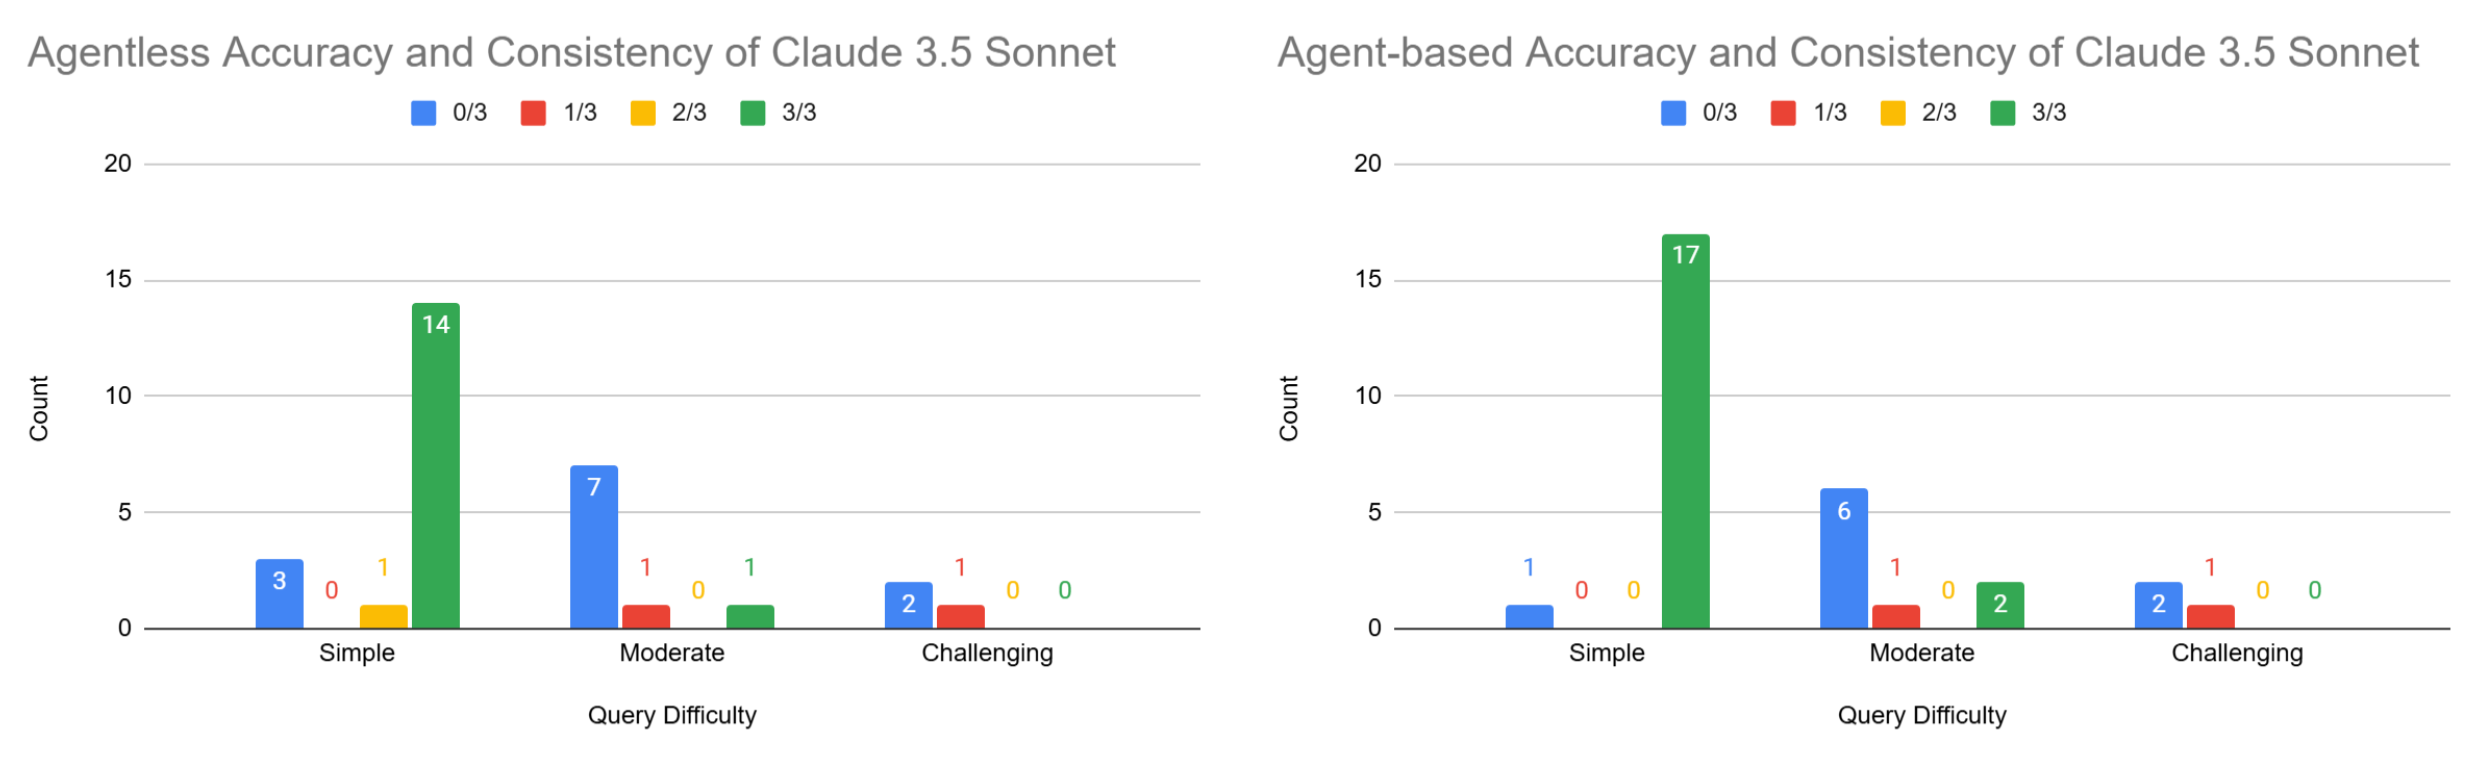
\includegraphics[width=\textwidth]{imgs/Claude Results Combined.png}
        \caption{Accuracy and Consistency of Claude 3.5 Sonnet}
        \label{fig:claude-results}
    \end{subfigure}
    \hfill
    % Second subfigure
    \begin{subfigure}[b]{0.45\textwidth}
        \centering
        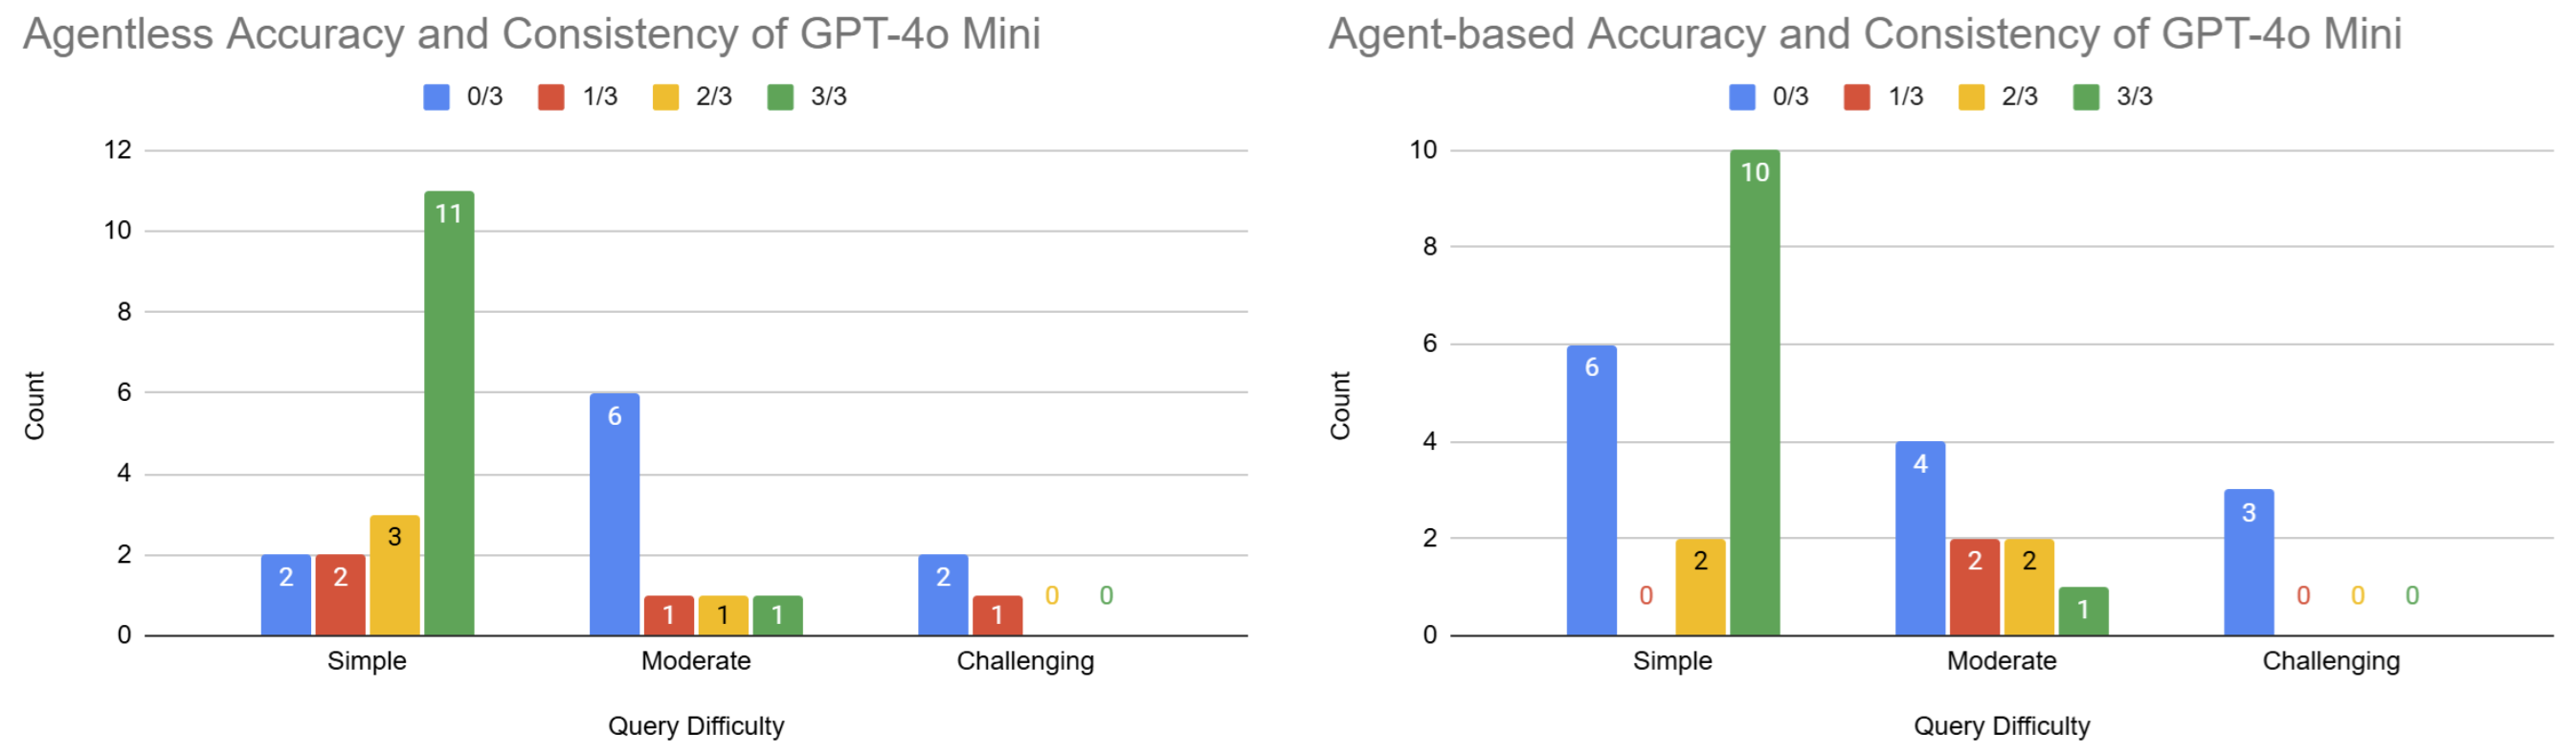
\includegraphics[width=\textwidth]{imgs/GPT Results Combined.png}
        \caption{Accuracy and Consistency of GPT-4o mini}
        \label{fig:gpt-results}
    \end{subfigure}
    \hfill
    % Third subfigure
    \begin{subfigure}[b]{0.45\textwidth}
        \centering
        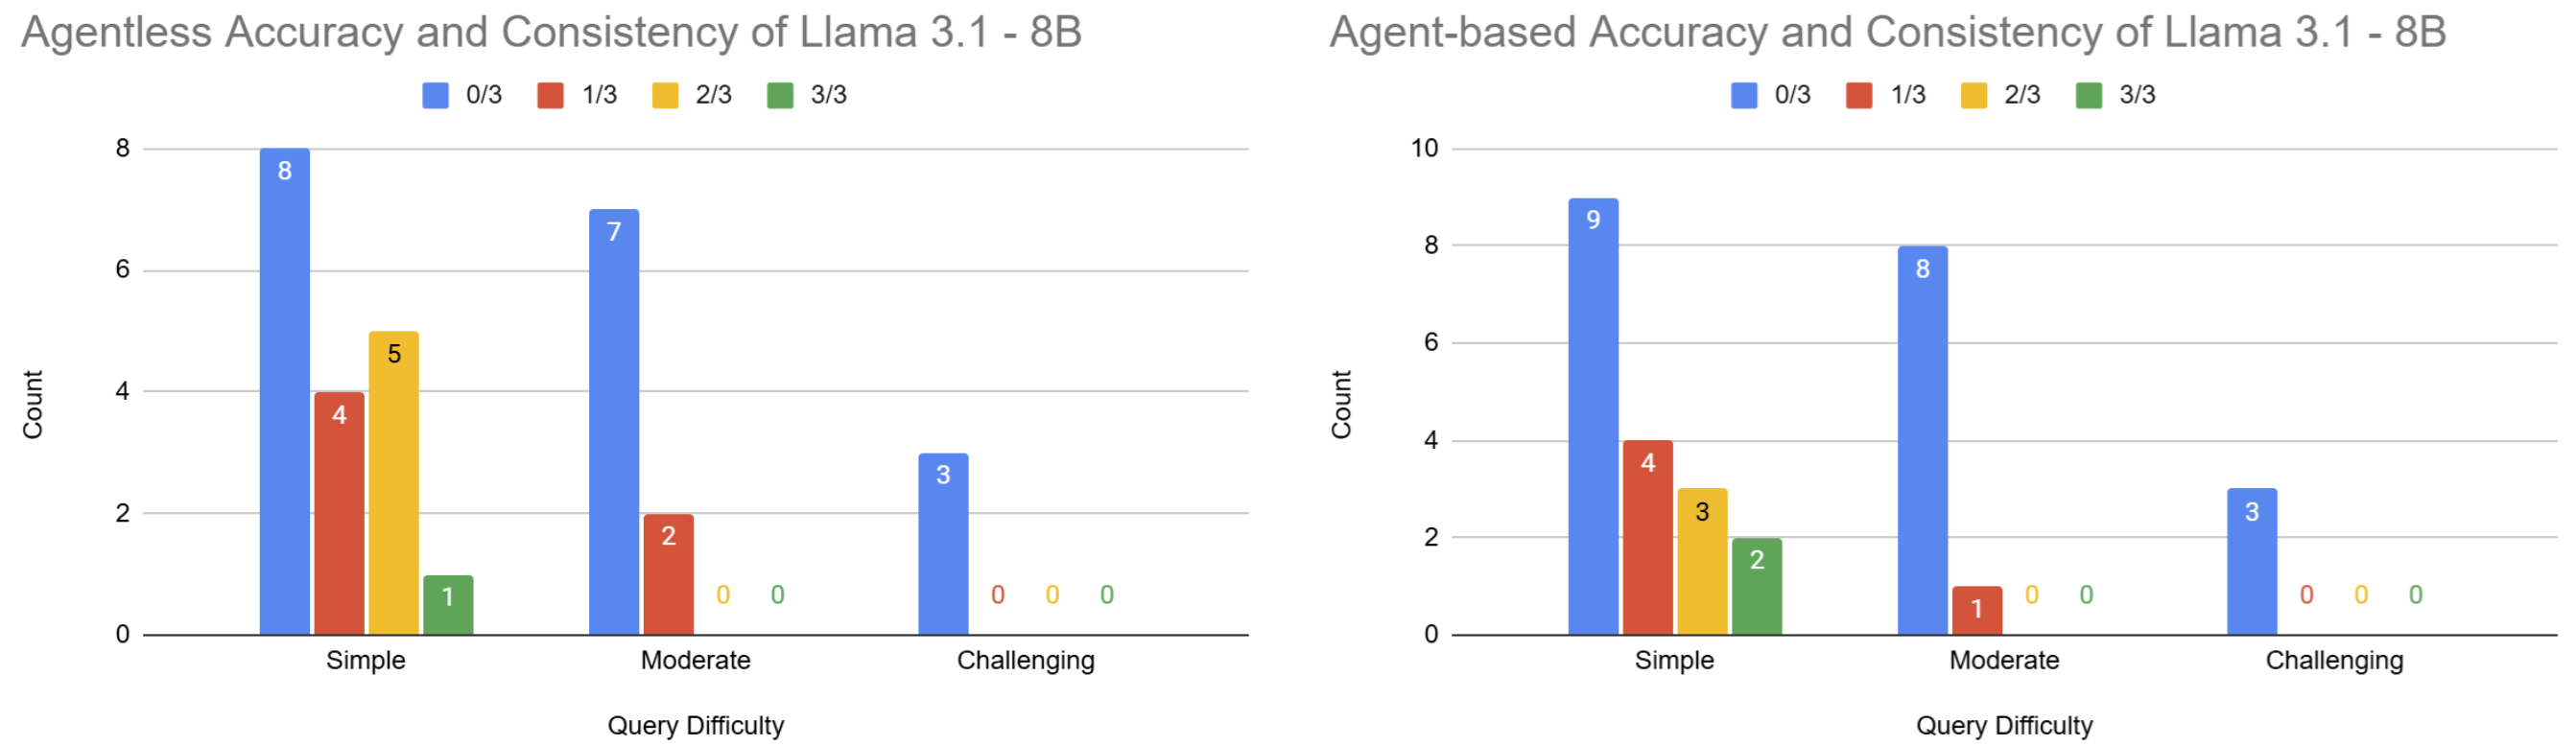
\includegraphics[width=\textwidth]{imgs/Llama Results Combined.png}
        \caption{Accuracy and Consistency of Llama3.1 8B}
        \label{fig:llama-results}
    \end{subfigure}
    % Overall caption
    \caption{Accuracy and Consistency}
    \label{fig:all-results}
\end{figure}

We evaluate the accuracy and consistency of each Model+Framework combination by generating a SQL query for each NLQ 3 times. Then we categorize the results into 4 buckets: 0/3, 1/3, 2/3, and 3/3 correct generations. The performance for each model under agentless and agent-based frameworks is summarized in Figure \ref{fig:all-results}.

Figure \ref{fig:claude-results} shows the accuracy and consistency results for Claude 3.5 Sonnet. Under the agent-based framework, Claude 3.5 Sonnet achieved near-perfect consistency on simple queries, with 17 out of 18 queries correctly answered 3 out of 3 times. However, for moderate queries, there was a notable drop in performance: 6 queries fell into the 0/3 category, indicating a struggle with moderately complex queries. Challenging queries were even more difficult, with only a few achieving any correct runs. In the agentless framework, performance remained strong but slightly lower than agent-based for simple queries, with 14 queries answered perfectly. Moderate and challenging queries showed a similar trend of decreased accuracy and consistency. Overall, Claude 3.5 Sonnet demonstrated the highest robustness among all models, especially on simple queries, with the agent-based framework offering a slight advantage.

Figure \ref{fig:gpt-results} shows the accuracy and consistency results for GPT-4o Mini. Unlike Claude, GPT-4o Mini showed more variability even on simple queries. Under the agent-based framework, only 10 out of 18 simple queries achieved 3/3 correctness, with 6 queries failing completely (0/3). Moderate queries exhibited mixed success, while challenging queries were unsuccessful. In the agentless framework, GPT-4o Mini's performance on simple queries slightly improved, with 11 queries answered perfectly. However, its performance on moderate queries worsened. Interestingly, its performance on challenging queries improved slightly where 1 query was answered correctly 1/3 times. Compared to Claude, GPT-4o Mini was less stable across runs, especially for more complex queries.

Figure \ref{fig:llama-results} shows the accuracy and consistency results for Llama3.1 8B, which was the least consistent of the three models. Under both frameworks, the majority of queries, including simple ones, fell into the 0/3 correctness category. Only a small number of queries achieved perfect correctness, primarily for easier queries. Moderate and challenging queries were particularly problematic, with most attempts failing across all runs. These results highlight the limitations of smaller or less refined models in structured generation tasks like Text2SQL.

Across all models, simple queries were solved more consistently than moderate and challenging ones. Claude 3.5 Sonnet was the most accurate and consistent model overall, with agent-based frameworks offering slight improvements. In contrast, GPT-4o Mini and Llama3.1 8B struggled more, suggesting that larger model size and training quality significantly influence Text2SQL performance. Additionally, there was no clear difference in performance between agentless and agent-based frameworks for GPT-4o Mini and Llama3.1 8B. Finally, GPT-4o Mini performs significantly better than Llama3.1 8B, even though they are approximately the same size. This suggests that factors beyond model size—such as training data quality, fine-tuning strategies, model architecture, and prompt alignment—play a critical role in determining a model’s ability to perform structured generation tasks like Text2SQL.

\subsection{Execution Error Comparison}

\begin{figure}[h]
    \centering
    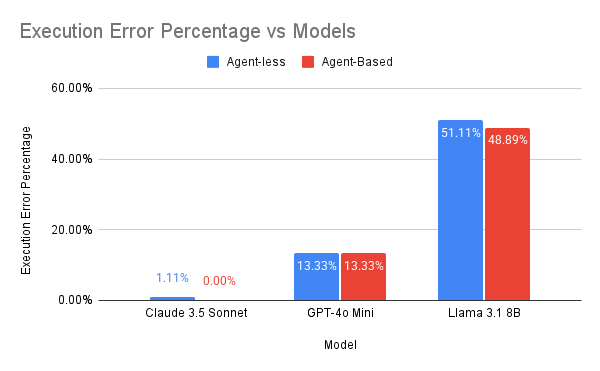
\includegraphics[width=0.45\textwidth]{imgs/Execution Error Percentage vs Models.png}
    \caption{Execution Error Comparison}
    \label{fig:execution-error-comparison}
\end{figure}

Execution error rates measure the proportion of generated queries that failed to run due to syntax errors, invalid table references, or other structural mistakes. Figure \ref{fig:execution-error-comparison} summarizes the execution error rates across models and frameworks.

Claude 3.5 Sonnet exhibited exceptional robustness, achieving an execution error rate of just 1.11\% under the agentless framework and 0.00\% under agent-based. This reflects highly reliable SQL generation. GPT-4o Mini exhibited moderate robustness, with an execution error rate of 13.33\% across both frameworks. Llama 3.1 8B had the highest execution error rates, exceeding 48\% under both frameworks. This highlights significant challenges in generating syntactically correct SQL, even before considering semantic correctness. Overall, larger and more capable models exhibited lower execution error rates, aligning with trends observed in correctness and consistency.

\subsection{Agentless vs Agent-based Performance}

\begin{figure}[h]
    \centering
    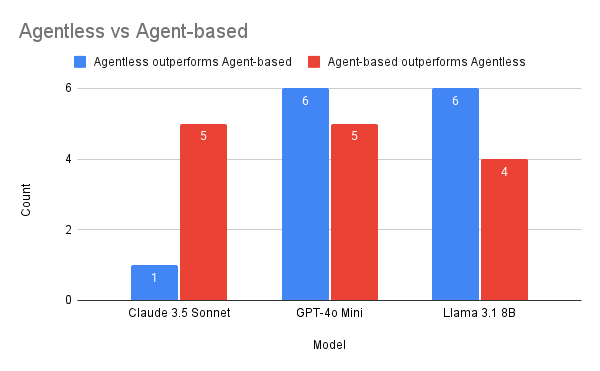
\includegraphics[width=0.45\textwidth]{imgs/Agentless vs Agent-based.png}
    \caption{Agentless vs Agent-based Comparison}
    \label{fig:framework-comparison}
\end{figure}

Finally, we compared the two frameworks directly by counting how often agentless or agent-based pipelines generated better results for a given query, summarized in Figure \ref{fig:framework-comparison}.

For Claude 3.5 Sonnet, the agent-based framework outperformed agentless in 5 queries, while agentless performed better in only 1 case. This suggests that Claude benefits from specialized agents that handle relevant table description extraction. For GPT-4o Mini, the agentless framework slightly outperformed agent-based (6 cases vs. 5). Similarly, for Llama3.1 8B, agentless was favored more often (6 cases vs. 4). Thus, for GPT-4o Mini and Llama3.1 8B, there isn't a clear advantage between using agentless vs agent-based frameworks.

Interestingly, Claude 3.5 Sonnet, being a larger model, performed better when paired with the agent-based framework. In contrast, GPT-4o Mini and Llama3.1 8B, both smaller models, showed no clear advantage between agentless and agent-based pipelines. However, it cannot be definitively concluded that larger models inherently benefit more from agent-based frameworks, because only one large model---Claude 3.5 Sonnet---was tested. As a result, it remains unclear whether the observed improvement is due to Claude’s larger size or some Claude-specific characteristics, such as its training data, fine-tuning methods, or architectural design. To better understand the relationship between model size and framework effectiveness, future work would need to evaluate additional large models to see if they exhibit similar performance differences between agentless and agent-based pipelines.

\section{Conclusion and Future Directions}

%------------------------------------------------------------------------- 
% \nocite{ex1,ex2}
\bibliographystyle{latex8}
\bibliography{latex8}

\pagebreak

\end{document}